\documentclass[twocolumn]{article}
\usepackage[utf8]{inputenc}
\usepackage{blindtext}
\usepackage[paperheight=252mm,paperwidth=174mm,margin=1mm,heightrounded]{geometry}
\usepackage{ulem}
\usepackage{listings}

\usepackage{minted}
%\BeforeBeginEnvironment{minted}{}
%\AfterEndEnvironment{minted}{}

\usepackage{tikz}
\usetikzlibrary{shapes.geometric, arrows}
\usetikzlibrary{positioning}

\usepackage{color}
\definecolor{light-gray}{rgb}{0.95,0.95,0.95}
\setminted{bgcolor=light-gray}  % this line causes the problem

\setlength{\parindent}{1mm}
\setlength{\parskip}{0mm}

\tikzstyle{string} = [rectangle, rounded corners, inner sep=2mm, text centered, draw=black, fill=red!30]
\tikzstyle{bytes} = [rectangle, rounded corners, inner sep=2mm, text width=, text centered, draw=black, fill=blue!30]
\tikzstyle{int} = [rectangle, rounded corners, inner sep=2mm, text width=,  text centered, draw=black, fill=green!30]
\tikzstyle{arrow} = [thick,->,>=stealth]

\begin{document}

\title{Handling strings in Python 3}
\date{}
%\maketitle
\section*{Strings \& bytes in Python 3}

You are building an exploit and, not being a barbarian, have switched from Python 2 to 3. One part of your exploit involves leaking an important address by dumping a chunk of memory. This chunk of memory contains a lot of random data but somewhere in the middle you know that there is a string "Här: "\footnote{Swedish for "here"} followed by the 4 bytes representing the little endian encoding on the address you are looking for. You copy some old Python 2 code that you have used for a similar situation:
\vspace*{-0.7\baselineskip}

\begin{minted}{python}
def extract_leaked_pointer(leak):
    marker = 'Här: '
    start = leak.find(marker)
    leak_start = start + len(marker)
    leak_data = leak[leak_start:leak_start+4]
    return struct.unpack('<I', leak_data)[0]
\end{minted}
\vspace*{-0.7\baselineskip}

Sadly, when running this, you get the following error:
\vspace*{-0.7\baselineskip}

\begin{minted}{text}
TypeError: argument should be integer
 or bytes-like object, not 'str'
\end{minted}
\vspace*{-0.7\baselineskip}

To solve this, you try to decode the leaked bytes into a string by adding this line to the code:
\vspace*{-0.7\baselineskip}

\begin{minted}{python}
leak = leak.decode('utf-8')
\end{minted}
\vspace*{-0.7\baselineskip}

Unfortunately, this doesn't work either and you are left staring at another error message:

\begin{minted}[breaklines]{text}
UnicodeDecodeError: 'utf-8' codec can't
 decode bytes in position 0-1: invalid 
 continuation byte
\end{minted}

In \sout{anger} your desire to develop as hacker, you turn to \sout{Twitter and complain about how Python 3 sucks} this article to understand how to reason about Python 3, strings, character encodings and arbitrary bytes.

The problem is that you are trying to interpret an arbitrary sequence of bytes as UTF-8 encoded data. This is the equivalent of trying to push a square peg through a round hole. It won't work. The following diagram shows what you are trying to do and where it goes wrong.
\vspace{1mm}

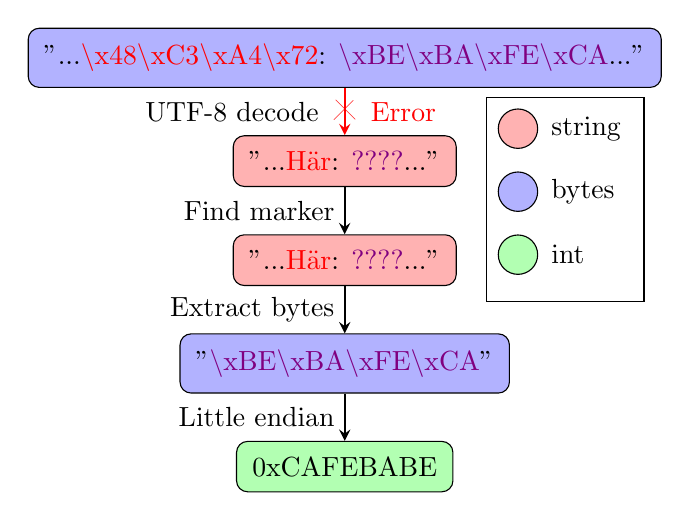
\begin{tikzpicture}

\node (in0) [bytes] {"...\textcolor{red}{\textbackslash x48\textbackslash xC3\textbackslash xA4\textbackslash x72}: \textcolor{violet}{\textbackslash xBE\textbackslash xBA\textbackslash xFE\textbackslash xCA}..."};
\node (in1) [string, below=6mm of in0] {"...\textcolor{red}{Här}: \textcolor{violet}{????}..."};
\node (in2) [string, below=6mm of in1] {"...\textcolor{red}{Här}: \textcolor{violet}{????}..."};
\node (in3) [bytes, below=6mm of in2] {"\textcolor{violet}{\textbackslash xBE\textbackslash xBA\textbackslash xFE\textbackslash xCA}"};
\node (in4) [int, below=6mm of in3] {0xCAFEBABE};


\draw [arrow,draw=red] (in0) -- node[color=red,pos=0.5,sloped,rotate=45]{|} node[color=red,pos=0.5,rotate=45]{|} node[anchor=east,xshift=-2mm] {UTF-8 decode} node[anchor=west,xshift=2mm,color=red] {Error} (in1);
\draw [arrow] (in1) -- node[anchor=east] {Find marker} (in2);
\draw [arrow] (in2) -- node[anchor=east] {Extract bytes} (in3);
\draw [arrow] (in3) -- node[anchor=east] {Little endian} (in4);

\draw [draw=black] (18mm,-5mm) rectangle (38mm,-31mm);
\draw [draw=black, fill=red!30] (22mm,-9mm) circle (2.5mm);
\node[anchor=west] at (25mm, -9mm) {string};
\draw [draw=black, fill=blue!30] (22mm,-17mm) circle (2.5mm);
\node[anchor=west] at (25mm, -17mm) {bytes};
\draw [draw=black, fill=green!30] (22mm,-25mm) circle (2.5mm);
\node[anchor=west] at (25mm, -25mm) {int};

\end{tikzpicture}

\vfill\null


Let's remind ourselves about character encodings. The goal is to represent a character such as "A". Computers work with numbers (more precisely bits), not characters, so we translate the character into a number. In the ASCII encoding, this is the number 65. We call this the codepoint. This value is then encoded using a single byte 0x41. This is simple in ASCII because there is a one to one to one mapping between characters, codepoints and bytes and this can be implicitly done without thinking about it. Python strings are not limited to ASCII but can represent the full Unicode range. If we use the UTF-8 encoding and take the character \textit{ä} we instead get:

\begin{table}[h]
\centering
\begin{tabular}{|l|l|l|l|}
\hline
Character & Codepoint & Bytes     & Encoding \\ \hline
A         & 65        & 0x41      & ASCII    \\ \hline
A         & 65        & 0x41      & UTF-8    \\ \hline
ä         & 228       & 0xC3 0xA4 & UTF-8    \\ \hline
\end{tabular}
\end{table}

\vspace*{-0.7\baselineskip}
Specifically, one character maps to a codepoint which is encoded with more than one byte and not every sequence of bytes represents a valid character. This is what causes the problem. To solve this, instead of trying to convert the "haystack" bytes into a string and search for a substring, you convert the "needle" marker into a sequence of UTF-8 bytes and search for that sequence of bytes in the haystack. When it is found, you can extract bytes relative to that offset and process them accordingly, in this case, convert them to a 32-bit number. This slightly modified diagram describes this approach.

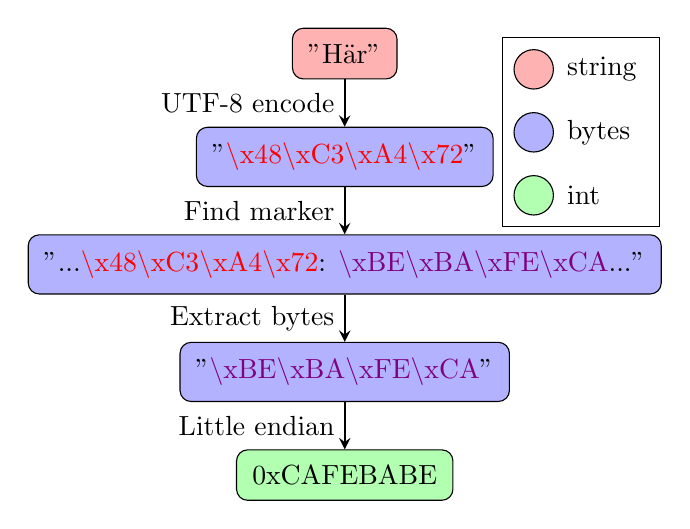
\begin{tikzpicture}

\node (in0) [string] {"Här"};
\node (in1) [bytes, below=6mm of in0] {"\textcolor{red}{\textbackslash x48\textbackslash xC3\textbackslash xA4\textbackslash x72}"};
\node (in2) [bytes, below=6mm of in1] {"...\textcolor{red}{\textbackslash x48\textbackslash xC3\textbackslash xA4\textbackslash x72}: \textcolor{violet}{\textbackslash xBE\textbackslash xBA\textbackslash xFE\textbackslash xCA}..."};
\node (in3) [bytes, below=6mm of in2] {"\textcolor{violet}{\textbackslash xBE\textbackslash xBA\textbackslash xFE\textbackslash xCA}"};
\node (in4) [int, below=6mm of in3] {0xCAFEBABE};


\draw [arrow] (in0) -- node[anchor=east] {UTF-8 encode} (in1);
\draw [arrow] (in1) -- node[anchor=east] {Find marker} (in2);
\draw [arrow] (in2) -- node[anchor=east] {Extract bytes} (in3);
\draw [arrow] (in3) -- node[anchor=east] {Little endian} (in4);

\draw [draw=black] (20mm,2mm) rectangle (40mm,-22mm);
\draw [draw=black, fill=red!30] (24mm,-2mm) circle (2.5mm);
\node[anchor=west] at (27mm, -2mm) {string};
\draw [draw=black, fill=blue!30] (24mm,-10mm) circle (2.5mm);
\node[anchor=west] at (27mm, -10mm) {bytes};
\draw [draw=black, fill=green!30] (24mm,-18mm) circle (2.5mm);
\node[anchor=west] at (27mm, -18mm) {int};

\end{tikzpicture}

Which, translated to Python 3 code, looks like this:

\begin{minted}{python}
def extract_leaked_pointer_python3(leak):
    marker = 'Här: '.encode('utf-8')
    start = leak.find(marker)
    leak_start = start + len(marker)
    leak_data = leak[leak_start:leak_start+4]
    return struct.unpack('<I', leak_data)[0]
\end{minted}

\vspace*{-0.7\baselineskip}
In short, don't try to convert bytes that don't represent text, into text. Instead convert the text into bytes, use it to extract the relevant bytes and then process them accordingly. Now your exploit works in Python 3 and you can leave another legacy language behind.

\end{document}
